\chapter{Background}
\label{chp:background}


This chapter will give a brief introduction to the history behind the BLOPP project (\ref{sec:bloppproject}) and the CAPP, GAPP and Karotz applications. 
Section \ref{sec:exisiting-products} gives an overview of some of the applications that are currently on the market, a brief look at some of them, in addition to an overview of an assessment that has been performed on the applications that are currently on the market.   
Section \ref{sec:existing-research} will give an introduction to some of the current research that has been performed on mobile technology in combination with children and health.   


\section{BLOPP Project}
\label{sec:bloppproject}
Barns LegemiddelOPPlevelser (BLOPP) is a project group working for ``Sykehusapotekene i Midt-Norge'' (Hospital pharmacies in Mid-Norway). Their purpose is to create easier medical treatments for children through use of technology.
%TODO:Bare skrive generelt om BLOPP her.
%TODO: Skal dette avsnittet være her?

\section{CAPP, KAPP and GAPP}
\label{sec:cappgappkapp}
In the autumn of 2012 Aaberg, Aarseth, Dale, Gisvold and Svalestuen were engaged by the BLOPP Project group through the course ``TDT4290 - Customer Driven Project'' \cite{customerdrivenntnu} at NTNU. During the period of August 2012 to December 2012 they developed a prototype of a mobile information system consisting of two applications and a tangible user interface. One application was developed for guardians of a child (GAPP), and two applications were developed for children (CAPP and KAPP). In this section, we discuss them further in detail, while a full report of their work is available at [Insert Reference].

Their prototype is the foundation for our work in this project.\footnote{The applications have norwegian as their main language} %Hvor kan vi putte dette?

\subsection{CAPP}
CAPP is an Android application targeted towards the children. It launches the alarms given by parents and guides children during their medication. When the alarm is launched, the medication process starts, where the child is taken through the process by an avatar in the application. 


One of the objectives towards CAPP was to introduce a gamification experience to the process. Accordingly, the child gets a golden star in his/her treasure chest once the child is done, however, these stars were not useful for anything else but showing them off.

As the target group for the application is children below the age of 8 it is reasonable to assume that not all of them are able to read, this application consists mainly of pictures.  
Figure \ref{fig:capp-main-menu} shows a screen shot of the main page. 

\begin{figure}
		\centering
			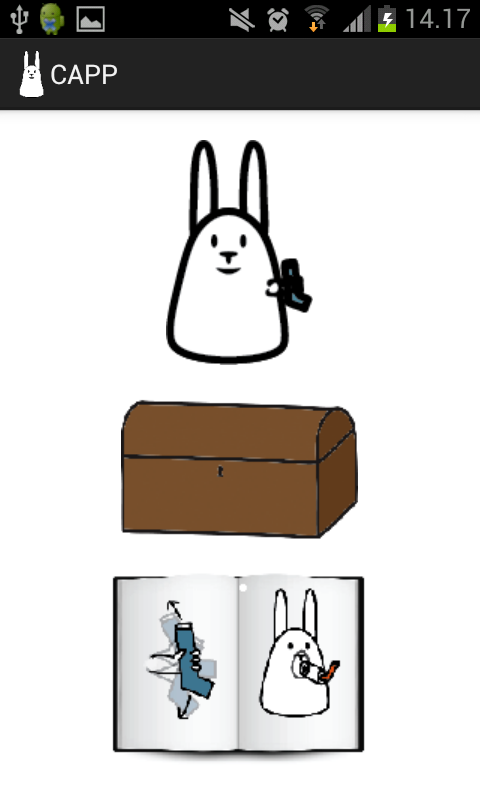
\includegraphics[width=0.20\paperwidth]{Pictures/app-screenshots/capp_main_menu.png}
		\caption{CAPP main menu}
		\label{fig:capp-main-menu}
\end{figure}



\subsection{KAPP}
KAPP is the other application targeted towards children. The application runs on a Karotz\cite{karotz}, which is a small robot bunny (see Figure \ref{fig:karotz}). The purpose of the Karotz is similar to CAPP, namely to remind children when it is time to take their asthma medicine and give instructions during treatment. In order to interact with the Karotz, children may use either a Nanoz (a small bunny with an integrated RFID) or by pressing a button on the top of the Karotz' head. In addition, it is possible to interact through the Karotz' ears, but from our part, this has not been experimented with.     

%TODO:BESKRIVELSE AV MEDISINERINGS PROSESS?


\begin{figure}
	\begin{minipage}[b]{0.4\linewidth}
		\centering
			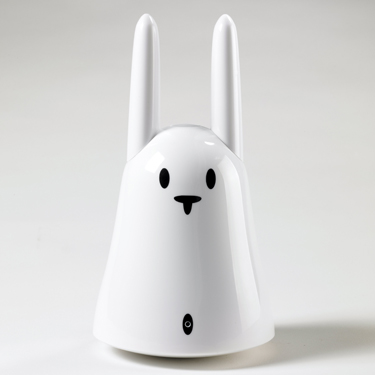
\includegraphics[width=0.20\paperwidth]{Pictures/karotz.jpg}
		\caption{Karotz}
		\label{fig:karotz}
	\end{minipage}
	\hspace{3cm}
	\begin{minipage}[b]{0.4\linewidth}
	\centering
		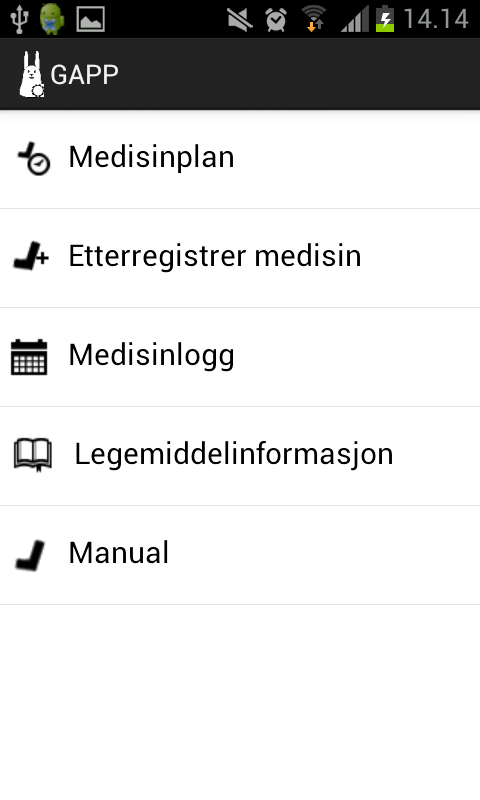
\includegraphics[width=0.20\paperwidth]{Pictures/app-screenshots/gapp_main_menu.png}
		\caption{GAPP main menu}
		\label{fig:gapp-main-menu1}
	\end{minipage}
\end{figure}


\subsection{GAPP}
GAPP is an Android application targeted towards the parents or guardians of the children. 
Currently, guardians are having problems with remembering how often their children have taken their medicine the last couple of days, when they should take them and how their child's desease has evolved the last couple of days. The purpose of GAPP is to let guardians monitor their child's medication usage the last couple of days, setting up reminders, etc.

Figure \ref{fig:gapp-main-menu1} shows a screenshot of the main menu of GAPP. The main functionality is separated into 
\emph{Medical Plan}, \emph{Register treatment}, \emph{Medicine log}, \emph{Information about the medicines} and \emph{Manual}. 
Medical Plan gives parents the option to set up reminders at particular times. 

The ``Register treatment''-option gives parents possibility to register a treatment that is taken in case the child forgot to go through the process in CAPP or KAPP. This way, children will be rewarded with stars accordingly. 
``Information about the medicines'' gives general information about different medicines, what they do, and what they are used for.  
``Medicine log'' shows how many times a child has taken their medicine the last couple of days.
The manual is to help ``newcomers'' to medicate children. For instance, if an aunt is watching children with asthma, then they could use the application as a reference on how to do the process. 
        
        
It's basic functionality is to view logs on how often a child needs medication, how the child has been feeling the last couple of days, according to the asthma traffic light system, and to set up alarms for the child. 
CAPP and GAPP work together as a pair, and thus the log will show the logged treatments of their child. 


\subsection{Known areas for improvement}
\label{sec:improvements}
As Aaberg et al. finished their work, they commented on several areas of potential improvement for CAPP/GAPP/KAPP. This document is reprinted in its entirety in Appendix \ref{app:furtherWork} (after permission from Aaberg, Aarseth, Dale, Gisvold and Svalestuen). The main topics for improvement were
\begin{itemize}
\item{Reward System}
\item{Distraction sequence for children}
\item{Web application}
\item{Support for more children}
\end{itemize}

Additionally, we want to use air quality data provided by \href{http://luftkvalitet.info}{Norwegian Institute for Air Research} 

These comments are used as a basis when we decide what to improve in this project. 
%TODO: Seksjon om modifikasjoner!


\section{Existing products}
\label{sec:exisiting-products}

On the two biggest application stores, Google Play and iOS AppStore, we have found a couple of applications similar to the one we have in mind. Among the ones we have looked into, is Huff and Puff \fnurl{Google Play : Huff And Puff}{https://play.google.com/store/apps/details?id=com.healthnutsmedia.huffandpuffsd.free}, Asthma Logger
\fnurl{Google Play : Asthma Logger}{https://play.google.com/store/apps/details?id=org.androworks.asthmalog}, Kids Beating Asthma \fnurl{Google Play : Kids Beating Asthma}{https://play.google.com/store/apps/details?id=es.medianet.hcsc01} and Asthma Monitor \fnurl{Google Play : Asthma Monitor}{https://play.google.com/store/apps/details?id=ch.imvs.unibas.asthma}. Common for all these applications is that they have one specific aim. For instance, Huff and Puff wants to teach children in general about asthma. Asthma Logger logs treatments, and Kids Beating Asthma have some game elements, but the games are not available for playing during treatment. For our product, we want to create a superset of these applications. 

\begin{sidewaystable}
	\label{tab:existing-product-table}
	\begin{tabular}{ | p{4.0cm} | p{5.5cm} | p{5.5cm} | p{4cm}|}
	\hline
	\textbf{Application} & \textbf{Positive} & \textbf{Negative} & \textbf{Target Audience} \\ \hline
	
   Huff And Puff 
	& 
	\begin{itemize}
	  \item Relevant quizzes from introduction to more experienced users
	  \item Can play sounds if children cannot read
	  \item Has asthma-specific word games, puzzles, etc.  
	\end{itemize}
	&
	\begin{itemize}
	  \item Poor navigation models
	  \item Quiz is too generic, for instance asks what doctors call this and that.
	  \item The games are not exactly what we look for, as they cannot be played while undergoing a treatment  
	\end{itemize}
	&
	Children
	\\ \hline
	Asthma Logger
	& 
	\begin{itemize}
	  \item Possibility to send journal on email specified by user. May forward the journal to doctor.  
	  \item Very intuitive application
	  \item Shows doses taken the last couple of days
	\end{itemize}
	& 
	\begin{itemize}
	  \item Only has one generic medicine (does not state which medicine, for instance Ventoline) or dosage (?) 
	\end{itemize}
	& 
	Adults
	\\ \hline
	Kids Beating Asthma
	& 
	\begin{itemize}
	  \item Informative and simple
	\end{itemize}
	&
	\begin{itemize}
	  \item Suffers from software bugs and crashes regularly
	\end{itemize}
	& Children
	\\ \hline
	Asthma Monitor
	&
	\begin{itemize}
	  \item Ability connect Peak Flow to activities
	  \item Thorough and ``advanced'' statistics
	  \item Can input symptoms like Cough, Sputum, Wheezing breath and Dyspnsea 
	  \item Can send records via email
	\end{itemize}
	&
	\begin{itemize}
	  \item Old fashioned GUI
	\end{itemize}
	& 
	Adults
	\\ \hline
	\end{tabular}
	\caption{Evaluation of existing products on the market}
\end{sidewaystable}

\subsection{Conclusion and evaluation}
\label{sec:existingconcl}

The main ideas we want to take further in our application are the email-sending system of Asthma Logger and the quiz-aspect of Huff And Puff. In general, it is a good idea to be able to send your journal on email, for instance to yourself. If we combine this with possibility to send the journal to a doctor, we have a great time saving tool. To give an example: Ole has been feeling ill for a while, and has been logging when he takes his medicine. He can then schedule an appointment with his doctor, and send his journal on email to the doctor. When he arrives to his appointment, the doctor already knows how many times he has taken his medicine the last days and can give advice based upon these facts. 

Asthma Monitor seems like a great application once you get used to it, and it is developed by researchers, which implies that they know what they're doing. However, it seems a bit too complex for the following reasons:
\begin{enumerate}
  \item If an adult who have no other experience of asthma other than through his/her child, the application contains terminology which they might not be very used to
  \item The user interface is not very appealing
  \item Forcing information from a child regarding how much they cough once a day seems rather hard 
\end{enumerate}   

As for the quiz, we have concluded that this is a great way to inform children. Namely by letting them playing around with the application and gathering knowledge on this basis. 

\subsection{Assessment of existing applications}
In 2012, Huckvale et. al. \cite{huckvale2012apps} conducted an assesment on the existing applications on both Google Play and AppStore. They assessed 103 different apps with english as the native language. Out of these 103, \emph{No apps for people with asthma combined reliable, comprehensive information about the condition with supportive tools for self­management.}(Huckvale et. al., 2012). They concluded that doctors should be careful when recommending apps for people with the purpose of self management. 






\section{Existing Research}
\label{sec:existing-research}

This section will give a foundation on some of the reserach performed on using technology in combination with diseases and children. 


\subsection{Monitoring Asthma with Mobile Technology}
There exists some research on self-management of monitoring your asthma condition. A lot of this research works used SMS (Short Messaging System) technology. In 2009, Andh\o j  et. al.\cite{anhoj2004feasibility} did a feasability study to check how users would respond to a SMS-reminder study. Their methodology was to send SMS a couple of times a day, and have the users respond to their peak flow and answer yes/no questions. Users could then access a web page to see different statistics on peak flows, how they've felt the last couple of days, etc.

They concluded that SMS is a feasible solution for collecting asthma diary data, mainly because the SMS technology was a big part of the participant's everyday life. Although SMS is a great technology to be used for this purpose, few children in our target group are able to use this technology, for obvious reasons. According to \emph{Senter for IKT i utdanningen} (Center for ICT in education), about 40\% of Norwegian children below the age of 3 years old have used a tablet, and 6 out of 10 children below the age of 6 have used a touch screen device \cite{nrkchilduse}. Thus the technological background should be somewhat familiar for our target group.  


\subsection{Children and Mobile Devices}
In 2013, \url{www.babies.co.uk} posted results on a poll they had posted on how many toddlers are using smartphones or tablets each day\cite{babiesusageoftablets}. Over 1000 participants responded,  and according to the survey, 14\% of the responders allowed children to use smartphones or tablets more than 4 hours a day. Considering the normal awake time of a child between 9 and 12 months old is approximately 10 hours, they spend a considerable amount of their day on the smartphone.         


\subsection{Children and Gestures}

Abdul Aziz et. al. \cite{aziz2013children} performed a study on which gestures children are able to comprehend when playing with an iPad. She tested 33 children's abililty to do gestures on a variety of applications suited for children. The children were in the range of 2-12 years old, 3 children per age. The study showed the following restrictions:

\begin{itemize}
  \item 2 year old children have difficulties with pinching, and are unable to drag and drop, spread and rotation of the device, and are not able to focus on the application. 
  \item 3 year old children have difficulties to drag and drop until they are told to do so, in addition to having problems with pinch and spread. 
  \item 4 year old children have difficulties to drag and drop. 
\end{itemize}
Children at age 5 and above are able to do all the normal gestures at a tablet. As CAPP is currently only available for mobile devices, this is reason for some discussion. The main part to notice is pinching and drag and drop. An iPad is fairly large relative to the size of these children's hands. There is reason to believe that gestures may be more difficult on smaller screens, however, we were unable to find research supporting this claim. In order to make AsthmAPP as child friendly as possible, it only uses ``swiping'' gestures and button presses for navigation.

\subsection{Assessment of Existing Applications}
In 2012, Huckvale et. al. \cite{huckvale2012apps} conducted an assesment on the existing applications on both Google Play\fnurl{Google Play}{http://play.google.com} and App Store\fnurl{Apple App Store}{http://www.apple.com/itunes/features}. They assessed 103 different apps with english as the native language. Out of these applications, 


\emph{``No apps for people with asthma combined reliable, comprehensive information about the condition with supportive tools for self­management''} \cite{huckvale2012apps}. 


They concluded that doctors should be careful when recommending apps for patients with the purpose of self management of asthma.


